\section{Libraries Design}

% Details on implementation.
% Architecture.

% TODO:
% - stunning architecture diagram
% - exciting example of usage
% - unbelievable python API showcase

\begin{figure}[t]
    \centering
    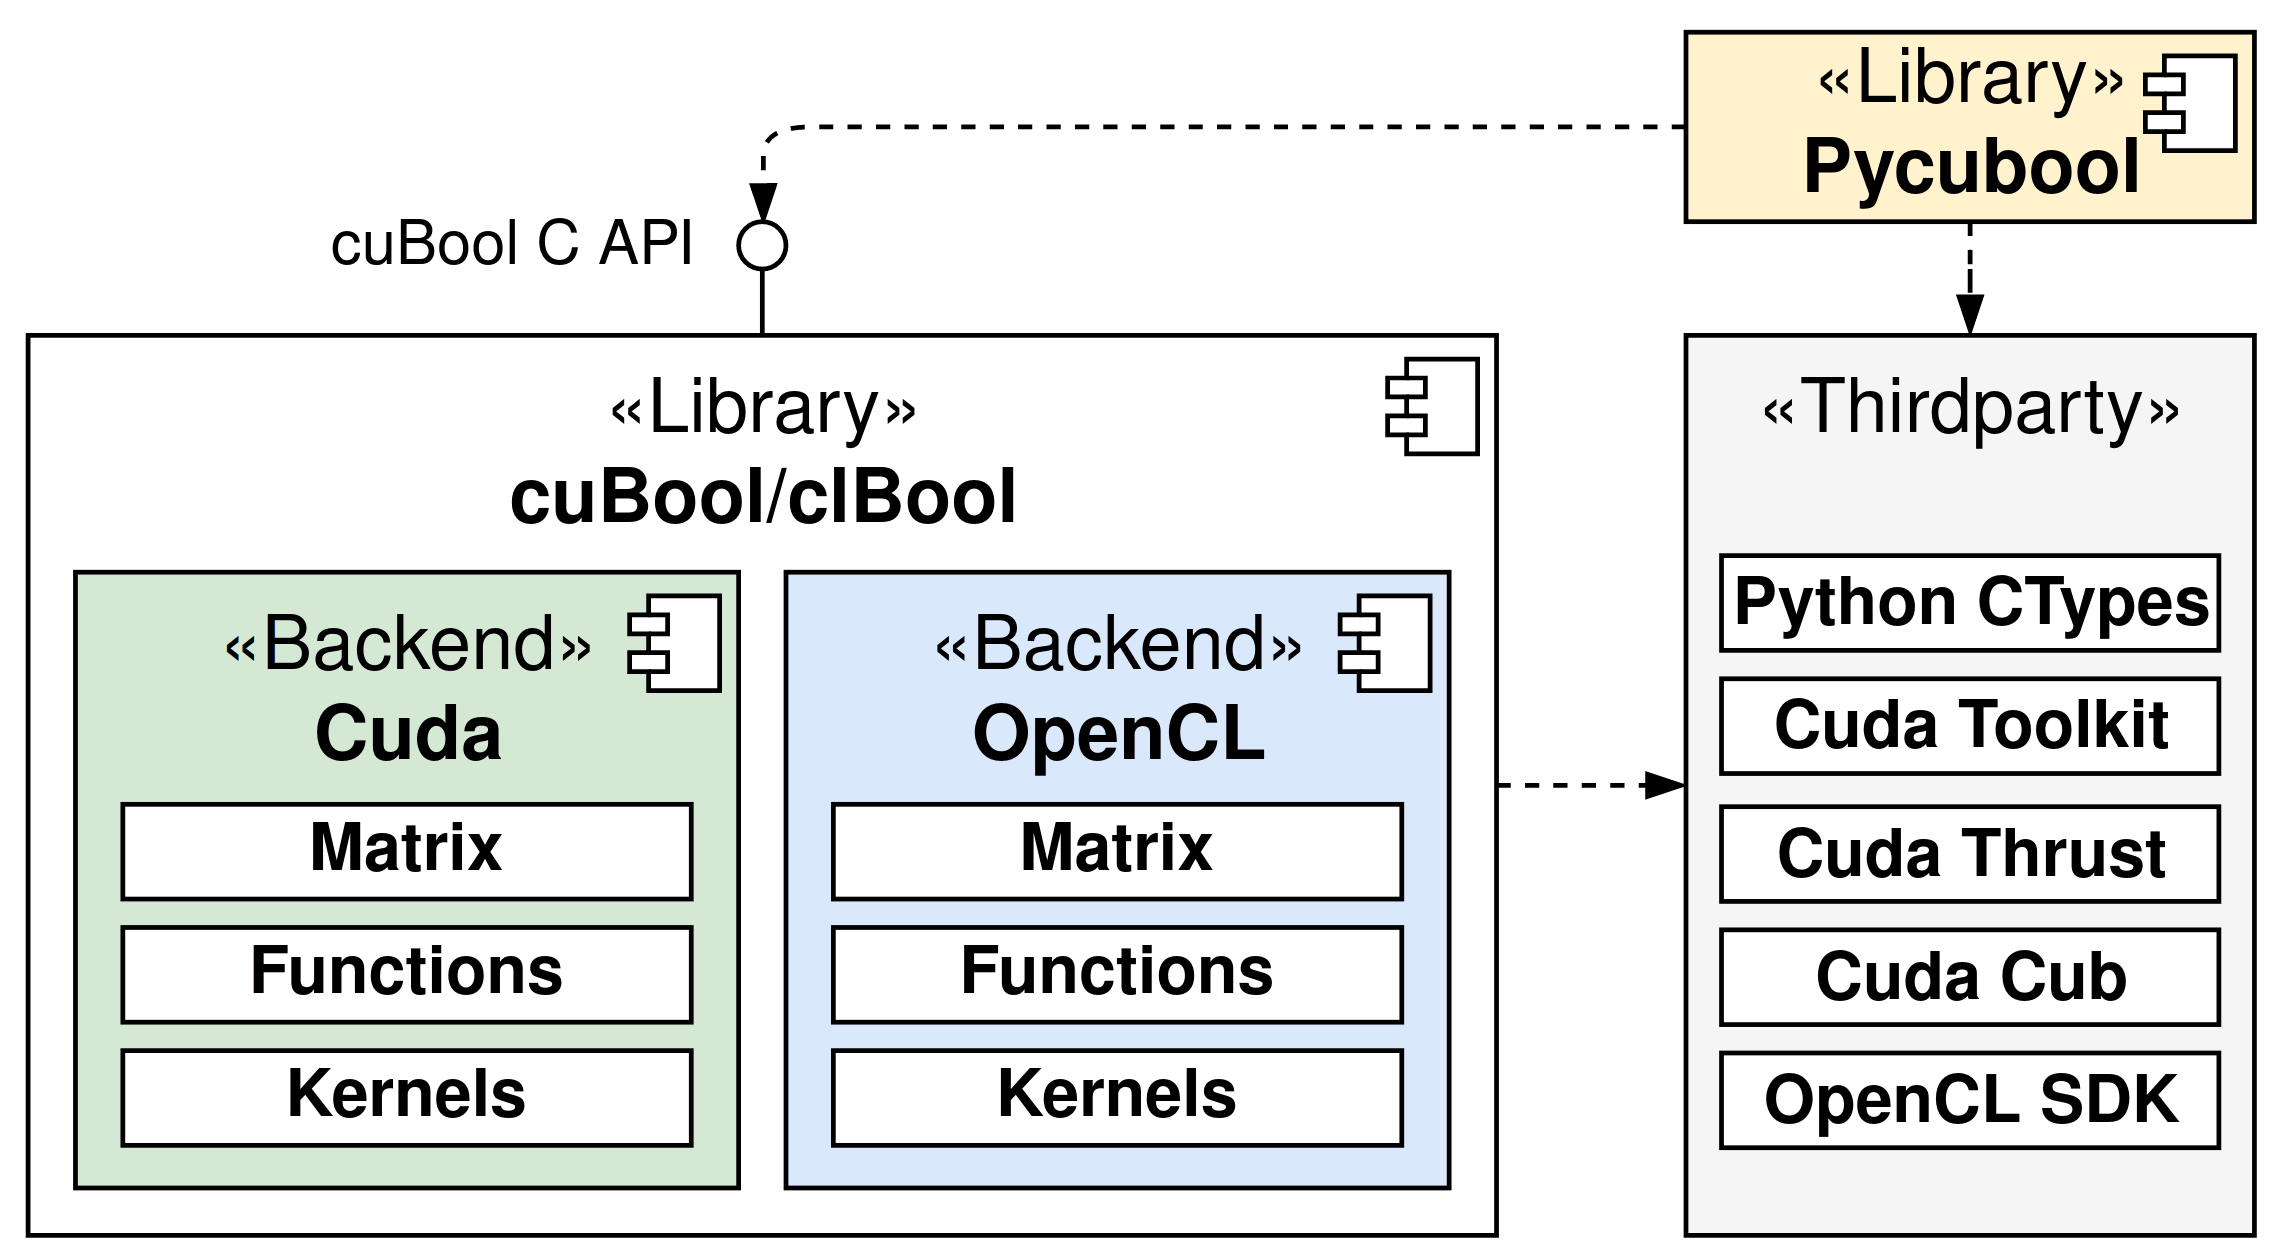
\includegraphics[width=0.39\textwidth]{generic_architecture.png}
    \caption{Sparse Boolean linear algebra library architecture.}
    \label{fig:generic_architecture}
\end{figure}

Implemented SPbLA library backends for NVIDIA Cuda and OpenCL platforms are called \textit{cuBool} and  \textit{clBool} respectively.
%%%%% I think, this info is too excessive. If you want to know something, go to the page with repos
% The projects are hosted on GitHub.
% The source code is licensed under MIT license.
% The build process is straightforward: it is configured with CMake tool and requires extra setup only for platform-specific development kits.
The general architecture of the SPbLA is depicted in figure~\ref{fig:generic_architecture}.
The core of the library is written in the C++ programming language, which is well-suited for performance and resource critical computational tasks.
The GPU related logic is in the platform specific backends.
% The GPU related logic is in the platform specific backends: Cuda and OpenCL, which use respective technologies for resources and GPU executable code management.
The library exposes C compatible API, which gives expressiveness and allows one to embed that API into other execution environments by interoperability mechanisms.
Pyspbla package encapsulates such functionality and provides it for the high-level Python runtime.

It is worth to mention, that the library is still being worked on. At this time clBool and cuBool are distinct backends, but they will be integrated into a single library.
This integration is planned for the near future.
This process requires careful selection of the interface to allow the end user to properly configure the library for specific tasks, as well as to provide the option to automatically select a specific implementation depending on the capabilities of the target device. 

However, cuBool already provides all the functionality described in the figure~\ref{fig:generic_architecture}.
It has a C compatible API, multiple backends for Cuda and CPU computations, a Python wrapper, and it is the lightweight version of the SPbLA without OpenCL computations.

Library operates on the boolean semiring with values set \{\textit{true}, \textit{false}\} with \textit{false} as an identity element, '$+$' operation is defined as logical \textit{or} and '$\times$' is defined as logical \textit{and}.
Values are also denoted as $\{1,~0\}$ respectively, and the abbreviation $\textit{nnz(M)}$ gives the number of non-zero cells of the matrix $M$.

The main primitive is a sparse matrix of boolean values, stored in one of the sparse formats.
The sparse vector is partially presented. 
Its full support will be added in the future. 
All available operations and functions are the following.

% \begin{itemize}
%     \item Create sparse matrix $M$ of size $m \times n$.
%     \item Delete sparse matrix $M$ and free all its internal resources.
%     \item Fill the matrix $M$ with values $L = \{(i,j)_k\}_k$. The result of this operation is $M_{i,j} = 1$ for each $(i, j) \in L$, and $M_{i,j} = 0$ otherwise.
%     \item \cho{Read matrix $M$ values $L = \{(i, j)~|~M_{i,j} = 1\}$.}
%     \item Matrix-matrix multiply-add operation $C \mathrel{+}= M \times N$.
%     \item Matrix-matrix add operation $M \mathrel{+}= N$.
%     \item Matrix-matrix Kronecker product $K = M \otimes N$.
% \end{itemize}

\begin{itemize}
    \item Create sparse matrix $M$ of size $m \times n$.
    \item Delete sparse matrix $M$.
    \item Fill matrix with values $\{(i,j)_k\}_k$.
    \item Read matrix values $\{(i, j)~|~M_{i,j} = 1\}$.
    \item Transpose $M = N^T$.
    \item Sub-matrix extraction $M = N[i..m, j..n]$.
    \item Matrix to vector reduce $V = \textit{reduceToColumn}(M)$.
    \item Matrix-matrix multiplication $C \mathrel{+}= M \times N$.
    \item Matrix-matrix element-wise addition $M \mathrel{+}= N$.
    \item Matrix-matrix Kronecker product $K = M \otimes N$.
\end{itemize}